\documentclass{article}[18pt]
\usepackage{../../../../format}
\lhead{Theory of Computation - Models of Computation}
\usepackage{mathrsfs}

\begin{document}
\begin{center}
\underline{\huge Advanced Topics in Computability}
\end{center}
\section{Diagonalisation}
\begin{defin}[Countable]
A set S is countable if there is a one-to-one correspondence between S and the set of natural numbers $\mathbb{N}$
\end{defin}
\section{Cantor's Proof}
\textbf{Proposition}: The set of reals in the interval (0,1) is uncountable\\
\\
\textbf{Proof}: A real number A in (0,1) is an (infinite) decimal expansion: $A=0.a_1a_2a_3...$\\
\\
Assume, for the sake of contradiction, there is a one-to-one correspondence between the real interval (0,1) and $\mathbb{N}$, i.e. all the reals in (0,1) can be ordered in a sequence
$$A_1,A_2,A_3...$$
We will construct a real number which is not in the sequence
\section{Cantor's diagonal argument}
Denote $A_i=0.a_1^ia_2^ia_3^i....$ and put the sequence in the following rectangular table
\[
\begin{array}{lllllllll}{A_{1}=} & {0} & {.} & {a_{1}^{1}} & {a_{2}^{1}} & {a_{3}^{1}} & {\ldots} & {\ldots} & {\cdots} \\
 {A_{2}=} & {0} & {\cdot} & {a_{1}^{2}} & {a_{2}^{2}} & {a_{3}^{2}} & {\ldots} & {\ldots} & {\cdots} \\
  {A_{3}=} & {0} & {\cdot} & {a_{1}^{3}} & {a_{2}^{3}} & {a_{3}^{3}} & {\ldots} & {\ldots} & {\cdots} \\
   {} & {\vdots} & {} & {} & {} & {\ddots} & {} \\
    {A_{i}=} & {0} & {.} & {a_{2}^{i}} & {a_{3}^{i}} & {\ldots} & {a_{i}^{i}} & {\cdots} & {\cdots} \\
     {\vdots} & {} & {} & {} & {} & {} & {\ddots} & {} \\
      {\vdots} & {} & {} & {} & {} & {} && {\ddots} \\
       {} & {} & {} & {} & {} &  & &&{\ddots}\end{array}
\]
Construct a new number $B=0.b_1b_2b_3...$ by taking
\[
b_{i}=\left\{\begin{array}{ll}{a_{i}^{i}+1} & {\text { if } a_{i}^{i}<9} \\ {0} & {\text { if } a_{i}^{i}=9}\end{array}\right.
\]
Now, B is a real number in (0,1) which is not in the table above, as $b_i\neq a_i^i$ for every i
\section{Halting problem by diagonalisation}
The set of all strings over a finite alphabet is countable - order them by length first and order the ones of the same length in lexicographic order
\[
\varepsilon, 0,1,00,01,10,11,000,001,010,011,100,101, \ldots
\]
Therefore, the set of all Turing machines is countable, too. Put all TMs vs all inputs in an infinite table.
\begin{center}
	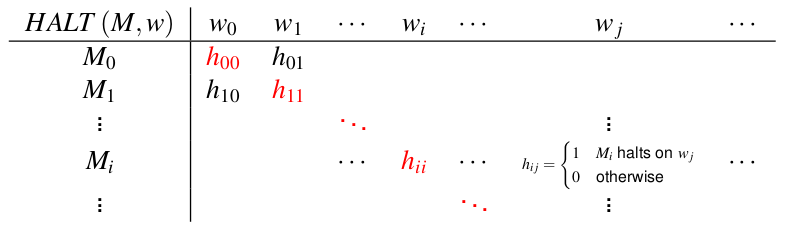
\includegraphics[scale=0.7]{Halting}
\end{center}
With the help of HALT machine, we created a TM M tat everywhere disagrees with the diagonal
\section{The class of Nice machines}
A set of Turing machines $\mathscr{N}$ has a Universal machine $U_{\mathscr{N}}(i,w)$ if
\begin{enumerate}
	\item For every machines $N\in \mathscr{N}$, there is a number $n$ such that $N(w)=U_{\mathscr{N}}(n,w)$ or all inputs $w$
	\item For every number $n$, the machine $U_{\mathscr{N}}(n,.)\in \mathscr{N}$
\end{enumerate}
\begin{defin}[Nice machines]
The class of "nice" machines $\mathscr{N}$ is the set of all TMs that terminate on every input
\end{defin}
\textbf{Proposition}: The class of "nice" machines $\mathscr{N}$ does not have a universal machine\\
\\
\textbf{Proof}: Assume that there is a universal function $U_{\mathscr{N}}(i,w)$. Diagonalise: consider the machine M defined by
\[
M\left(w_{i}\right)=\neg U_{\mathscr{N}}\left(i, w_{i}\right)
\]
for all i\\
\\
M itself is a nice machine, so there much be a number $n$ such that $M(w)=U_{\mathscr{N}}(n,w)$ for all inputs $w$. In particular, for $w=w_n$ we would have that
\[
M\left(w_{n}\right)=U_{\mathscr{N}}\left(n, w_{n}\right)
\]
However, but by the construction of M we have that
\[
M\left(w_{n}\right)=\neg U_{\mathscr{N}}\left(n, w_{n}\right)
\]
which is a contradiction
\section{Self-Reference}
We want a program (Turing machine) that ignores the input and produced its own source code (description) as output.
\begin{defin}[Quine]
A program that generates a copy of its own source code as its complete output
\end{defin}
\section{Solution by mutual recursion}
A quine that consists of two parts: A followed by B. A prints out B in a straightforward way, and then B prints out A using the output that has just been produced by A.
\begin{center}
	\includegraphics[scale=0.7]{"Mutual Recursion"}
\end{center}


\end{document}